% =============================================================================
% CAPÍTULO 11 — volta 3 (AGENTS.md §6): a geometria do condicionamento.
%
% O fracasso que o abre, com número na mão: a taxa de rompimento deixa 34 de 36 explicações
% caberem nos mesmos dados — e o pior bloco de 60 dias não deixa nenhuma, porque a família de
% duas leis sem memória só alcança 11 contra os 20 do dado.
%
% Medição: lab/experimentos/E07_condicionamento.ipynb e lab/experimentos/E47_projecao.ipynb. Figuras: figuras/E07_condicionamento_* e figuras/E47_projecao_*.
% =============================================================================

\chapter{Quantas explicações cabem}
\label{cap:condicionamento}

\section{A pergunta que o capítulo anterior deixou}

O capítulo anterior terminou com um empate suspeito: no mesmo orçamento, o alerta clássico e o
posto do corte anunciaram a rampa quase no mesmo dia --- e os dois bebem da mesma janela de
passado, de modo que talvez não sejam dois instrumentos. A suspeita é a de sempre, dita agora
com janela na mão: um pedaço finito de passado carrega uma quantidade finita de informação, e
essa quantidade pode não dar para tudo o que se quer
perguntar\cite{masry1996minimum,paninski2003estimation}.

Este capítulo mede essa quantidade com uma conta grosseira e direta. Toma-se uma família de
explicações --- todas as séries que se pode gerar com duas leis, uma calma e uma agitada ---, e
pergunta-se quantos membros da família reproduzem o que o dado mostra. A resposta tem duas
formas, e confundi-las é o erro que o capítulo persegue:

\begin{itemize}[leftmargin=1.5em]
  \item a estatística deixa uma \textbf{região}: muitas explicações cabem, e o dado não escolhe
    entre elas;
  \item a estatística corta o conjunto \textbf{a zero}: nenhuma explicação cabe, e o dado
    refutou a família inteira.
\end{itemize}

As duas são informação. A primeira diz o que ainda não se sabe; a segunda diz que a família
estava errada. Uma média entre as duas não diz nada.

\section{A família mais simples que existe}

A família tem dois parâmetros. O primeiro é \emph{p}, a fração de dias que passam no regime
agitado. O segundo é a razão entre as duas leis: quantas vezes o dia agitado é mais
agitado que o calmo. A oscilação global é mantida fixa em todos os membros, de modo que comparar
dois deles compare o mecanismo e não o tamanho.

O dado é a mesma série dos capítulos anteriores, com \numCondicionamentoDias{} dias, e as quatro
estatísticas que ele mostra: a taxa de rompimento de \numCondicionamentoTaxa, o pior bloco de
sessenta dias com \numCondicionamentoPior{} rompimentos, a mediana dos blocos em
\numCondicionamentoMediana, e a fração de blocos acima do dobro da promessa, que é de
\numCondicionamentoAcimaDoDobro. Um membro entra no conjunto quando as quatro cabem nas suas
tolerâncias: dois décimos de ponto percentual na taxa, dois rompimentos no pior bloco, um dia na
mediana e três centésimos naquela fração.
% aterramento: tolerancia
Uma \textbf{tolerância} é o erro que ainda se aceita entre duas contas para dizer que elas
concordam. Ela é uma decisão, e não uma medida do dado, e por isso se declara junto do número que julga.
Aqui são quatro, uma por estatística, e cada uma na unidade da estatística que ela mede --- dois
décimos de ponto percentual não é pouco nem muito até se saber que a taxa é de cinco por cento.

A primeira estatística é a do corte, e mede o nível. As outras três medem a forma com
que os rompimentos chegam, e é na forma que as explicações se separam.

\section{Com a taxa sozinha, quase tudo cabe}

A grade tem \numCondicionamentoCombinacoes{} membros. Exigindo apenas a taxa, dentro de uma
tolerância de dois décimos de ponto percentual, cabem \numCondicionamentoCabemTaxa{} deles.

Vale ler esse número devagar. \numCondicionamentoCabemTaxa{} explicações diferentes --- com frações agitadas
distintas e razões distintas entre as leis --- reproduzem o mesmo número que o corte discutiu. A promessa, sozinha, não identifica nada; ela é compatível com quase
toda a família. E isso não é defeito da família, é o que a estatística carrega: uma média não
guarda a forma.

\section{O pior bloco esvazia o conjunto}

Acrescentando o pior bloco de sessenta dias, o número que cabem passa a
\numCondicionamentoCabemTaxaPior{}.

O conjunto fica vazio, e não apenas pequeno. A família de duas leis, com
o estado sorteado de novo a cada dia, \textbf{não alcança} o agrupamento que o dado tem, e o teste é
direto: o melhor pior bloco que qualquer membro consegue produzir é de
\numCondicionamentoMelhorPior{} rompimentos, contra os \numCondicionamentoPior{} do dado.

Há uma coincidência que não é coincidência. Quando o capítulo do corte submeteu duzentos mundos
que nunca mudam à mesma rotina, o pior bloco de todos eles parou em \numNuncaMudaPiorBloco. A família medida chega perto desse teto sem alcançá-lo, e pelo mesmo motivo: sem memória, os dias ruins não têm como se
agrupar.

\begin{figure}[htbp]
  \centering
  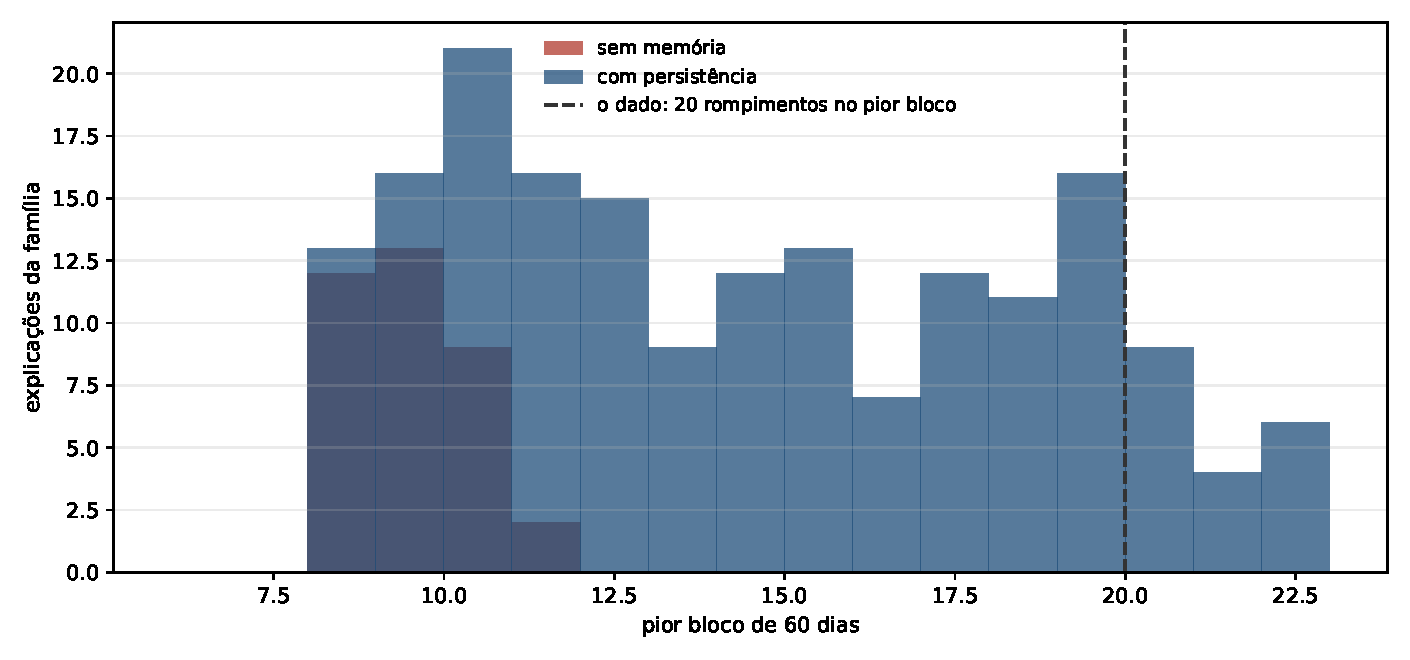
\includegraphics[width=\linewidth]{figuras/E07_condicionamento_1.pdf}
  \caption{Até onde cada família alcança o agrupamento do dado. A linha tracejada é o pior bloco
    que a série produziu; as barras são quantos membros de cada família chegam a cada valor. O vazio
    entre as barras da esquerda e a linha parece margem apertada na escala do desenho; é um muro, e
    não uma folga --- e onde as duas famílias caem no mesmo valor, a barra mais alta esconde a outra.}
  \label{fig:alcance}
\end{figure}

\section{O estado que dura}

O que falta à família é a única coisa que o dado parece exigir: que o regime dure. Um terceiro
parâmetro entra, e ele é a permanência média do regime agitado, em dias. Com permanência de um
dia o dia agitado nunca é seguido de outro, e a família fica mais arrumada que a sem memória.

A grade passa a \numCondicionamentoPersistenteCombinacoes{} membros, e a resposta muda de
natureza. Com a taxa sozinha cabem \numCondicionamentoPersistenteCabemTaxa\cite{jsang2007cumulative}. Com a taxa e o pior
bloco, cabem \numCondicionamentoPersistenteCabemTaxaPior{}. Com as quatro estatísticas, cabem
\numCondicionamentoPersistenteCabemQuatro{} --- dois membros da família inteira, com permanências
curtas, da ordem de dez a trinta dias. E esse número é de \emph{uma} varredura: repetida
\numCondicionamentoRepeticoes{} vezes, ele vai de \numCondicionamentoCabemQuatroMenor{} a
\numCondicionamentoCabemQuatroMaior{}, mediana \numCondicionamentoCabemQuatroMediana{} --- a
contagem de membros é do sorteio tanto quanto do dado, e o que se lê dela é a ordem de grandeza.

E o teto some: o melhor pior bloco que a família persistente alcança é de
\numCondicionamentoPersistenteMelhorPior{} rompimentos, que já cobre o que o dado mostra. O
excesso de blocos cheios também aparece, e até com folga: o maior valor da família é de
\numCondicionamentoPersistenteMelhorExcesso, contra \numCondicionamentoAcimaDoDobro{} do dado.

Uma explicação que reproduz as quatro estatísticas de uma série de \numCondicionamentoDias{} dias com dois
parâmetros e uma permanência é pouco. Duas explicações que as reproduzem são o resultado honesto
da medição: o dado identifica uma \textbf{região}, e não um ponto\cite{derr2023systems}.

\begin{figure}[htbp]
  \centering
  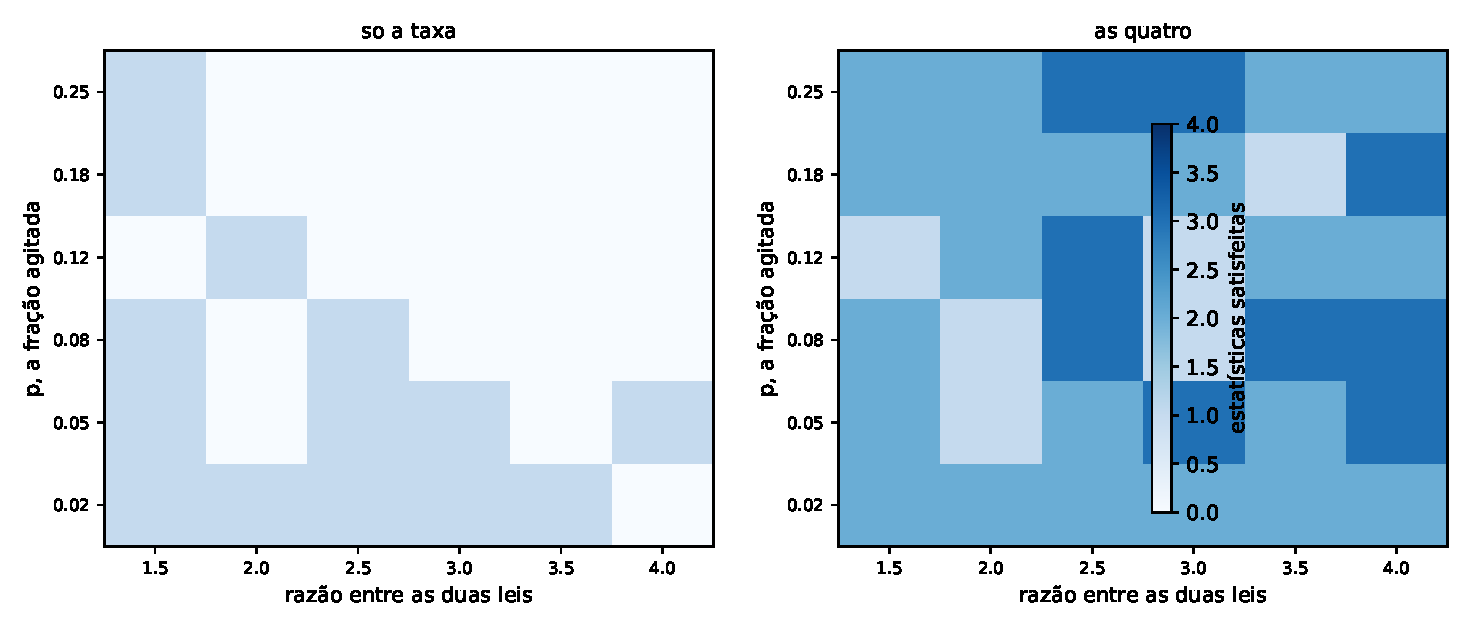
\includegraphics[width=\linewidth]{figuras/E07_condicionamento_2.pdf}
  \caption{O conjunto factível no plano dos dois primeiros parâmetros, para a permanência longa.
    À esquerda, os pontos que reproduzem a taxa; à direita, quantas das quatro
    estatísticas cada ponto satisfaz. A cor conta estatísticas satisfeitas, e não quão bom é o
    ajuste: escuro não é aprovação --- \numCondicionamentoPontosAsQuatro{} pontos da permanência
    mais longa chegam às quatro, e as \numCondicionamentoPontosSoATaxa{} da esquerda são as mais pálidas da escala.}
  \label{fig:factivel}
\end{figure}

O mapa da \cref{fig:factivel} diz o mesmo em duas dimensões. Na permanência mais longa,
\numCondicionamentoPontosSoATaxa{} dos \numCondicionamentoCombinacoes{} pontos do plano reproduzem a taxa, e \numCondicionamentoPontosAsQuatro{} reproduzem as quatro estatísticas --- o que confirma,
por outro caminho, que as duas explicações que sobrevivem têm permanência curta.

\section{O tamanho da região é de quem mede}

Falta o controle que separa o que é do dado do que é da minha escolha. A tolerância foi escolhida
por mim, e uma tolerância frouxa admite mais explicações por construção. E são quatro, uma por
estatística e na unidade da própria estatística: dois décimos de ponto percentual na taxa, dois
rompimentos no pior bloco, um dia na mediana e três centésimos na fração de blocos cheios. A conta foi repetida com
a tolerância apertada pela metade e com o dobro dela.

O veredito sobre a família sem memória não se move: \numCondicionamentoApertadaSemMemoriaTaxaPior{}
membros com a tolerância apertada, \numCondicionamentoEscolhidaSemMemoriaTaxaPior{} com a
escolhida e \numCondicionamentoFrouxaSemMemoriaTaxaPior{} com a frouxa. A refutação é do dado.

O tamanho do conjunto factível da família persistente, esse, depende da escolha:
\numCondicionamentoApertadaPersistenteQuatro{} explicações com a tolerância apertada,
\numCondicionamentoEscolhidaPersistenteQuatro{} com a escolhida e
\numCondicionamentoFrouxaPersistenteQuatro{} com a frouxa. Dizer "o dado identifica duas
explicações" sem dizer com que tolerância é dizer um número que pertence a quem mediu.

Vale a distinção, porque ela reaparece em tudo o que vem: \textbf{refutação é do dado; tamanho de
região é do critério}. O capítulo do corte já tinha mostrado a versão disso numa estatística só
--- o corte assina a média ---, e aqui ela aparece na forma completa.

\section{O peso de cada explicação}

O capítulo responde \emph{quantas} peças da família reproduzem as quatro estatísticas do dado:
\numEvidenciaCabem{}, das \numEvidenciaPecas{}. Ele não responde \emph{com que folga} cada uma
cabe, e a diferença importa: um empate de verdade e uma ordem com folga pequena têm a mesma cara
numa contagem.

A folga de uma peça é a distância à fronteira da tolerância, medida na unidade de cada estatística
--- de modo que \emph{um} é estar na borda e meio é ter metade do que se aceita. Medidas assim, as
duas que cabem não cabem igual: a primeira fica a \numEvidenciaFolgaPrimeira{} e a segunda a
\numEvidenciaFolgaSegunda, \textbf{exatamente na fronteira}, enquanto a primeira que fica de fora
está a \numEvidenciaFolgaTerceira. A razão entre as duas que entram é de
\numEvidenciaRazaoDuas{}, e da segunda até a que fica de fora é de \numEvidenciaRazaoFronteira.

\begin{figure}[htbp]
  \centering
  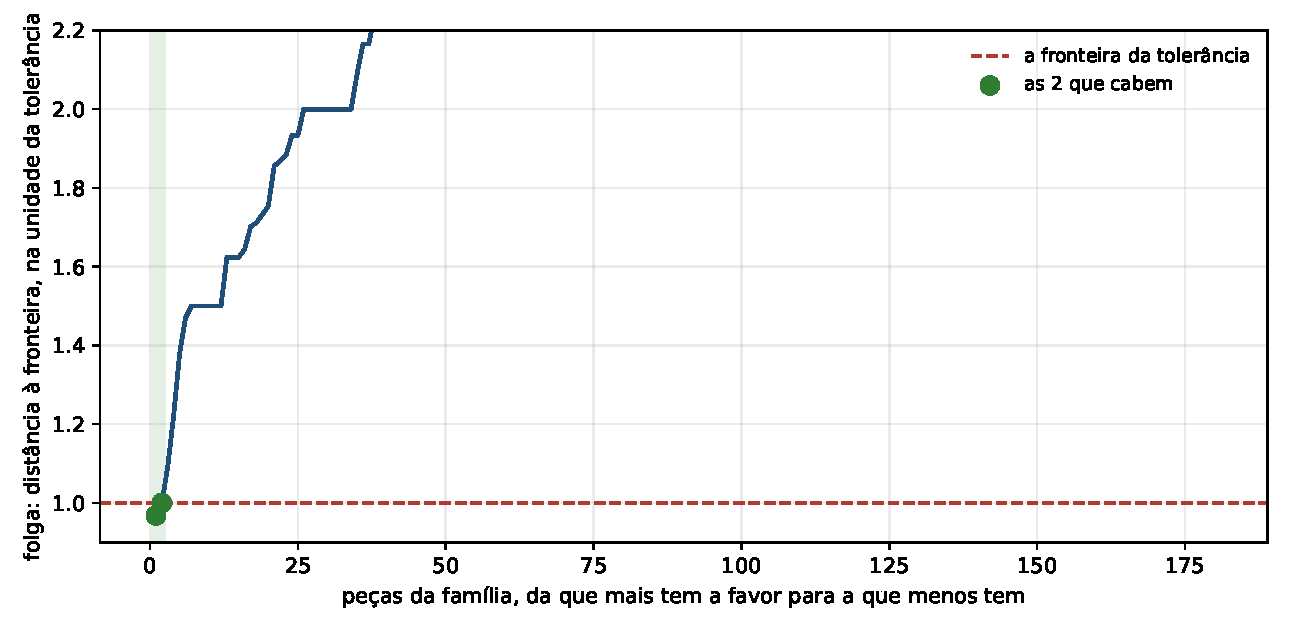
\includegraphics[width=\linewidth]{figuras/E25_evidencia_1.pdf}
  \caption{A folga de cada peça da família, da que mais tem a favor para a que menos tem. A linha
    tracejada é a fronteira da tolerância e a faixa verde, as \numEvidenciaCabem{} peças que o
    capítulo conta. A mais distante das \numEvidenciaPecas{} está a
    \numEvidenciaFolgaDistante{} tolerâncias.}
  \label{fig:folga}
\end{figure}

O que isso acrescenta à contagem é uma medida do quanto a fronteira decide. As duas peças que entram
estão separadas por três por cento da tolerância, e a segunda está em cima da linha: apertar a
tolerância um décimo a tira da conta. \textbf{O empate não é um empate: é uma ordem estreita
encostada na borda do critério} --- e é por isso que o capítulo declara a tolerância junto do número
que ela julga.

\section{A explicação que a divergência escolhe}

As quatro estatísticas do capítulo --- a taxa, o pior bloco, a mediana e o acima do dobro ---
são todas funcionais da \emph{mesma} lei: a lei empírica das contagens de rompimento por bloco de
\numBlocoDias{} dias. A taxa é a média dela dividida pelo bloco, o pior bloco é o máximo, a
mediana é o meio e o acima do dobro é uma cauda. A tolerância pergunta a quatro funcionais dessa
lei, uma de cada vez; nenhuma das quatro pergunta pela lei inteira. E é a lei inteira que o dado
mede.

% aterramento: divergencia
Para perguntar pela lei inteira é preciso uma régua entre leis, e a régua natural é a
\textbf{divergência de informação}: $D(p\\|q) = \sum p \ln(p/q)$, a soma sobre as casas da contagem, em
\emph{nats}. Ela vale zero quando as duas leis são a mesma e cresce quando uma se afasta da
outra; e ela não sabe nada de tolerâncias --- compara leis, não funcionais.

% aterramento: envoltoria
% aterramento: projecao
A família da grade já é um conjunto de leis. O fecho dela por mistura --- a \textbf{envoltória
convexa}, tudo o que se obtém ponderando os membros --- é o que a geometria pede, porque a
mistura de duas explicações ainda é uma explicação. A \textbf{projeção em divergência} de uma
lei sobre esse conjunto é o membro --- ou a mistura --- mais próximo dela, e ela existe e é
\emph{única}, porque o conjunto é convexo e a divergência é convexa nele: a canonicidade não é
escolha de quem mede, é propriedade da geometria \cite{csiszar1975divergence}.
% aterramento: desigualdade-de-pitagoras
A desigualdade de Pitágoras da divergência sustenta essa canonicidade: a distância de uma lei à família se decompõe na distância dela até o projetado mais a do projetado até qualquer outro membro, de modo que o projetado é o mais próximo de todos.

Feito isso \numProjecaoReplicas{} vezes --- cada réplica re-sorteia a grade inteira e refaz as
folgas, porque a escolha da tolerância é do sorteio tanto quanto do dado ---, as duas escolhas não
coincidem. A distância entre elas é de \numProjecaoDistanciaNats{} nats por bloco, medida da
escolha da tolerância para a escolha da geometria. O ponto escolhido não é um vértice solitário: o
peso do membro dominante é \numProjecaoPesoDominante{}, chegando a \numProjecaoPesoDominanteMax{}
na réplica mais decidida --- a escolha é uma mistura, quase sempre. O vértice dominante é o mesmo
em \numProjecaoVerticeEstavel{} das \numProjecaoReplicas{} réplicas.

Há uma assimetria que o número esconde e que a prosa tem de dizer. A escolha da tolerância deixa
casas do alfabeto sem massa nenhuma --- casas que o dado visita e ela não ---, e contra essas
casas a divergência na direção contrária é infinita. É por isso que a distância se mede num
sentido só, da escolha da tolerância para a projetada: \numProjecaoEscolhaCasasZero{} casas por
réplica, e em \numProjecaoEscolhaFora{} das \numProjecaoReplicas{} réplicas essa escolha visita
casas onde o dado tem massa e ela não. A projeção, por construção, não faz isso: ela é obrigada a
responder a todas as casas em que o dado responde.

\begin{figure}[htbp]
  \centering
  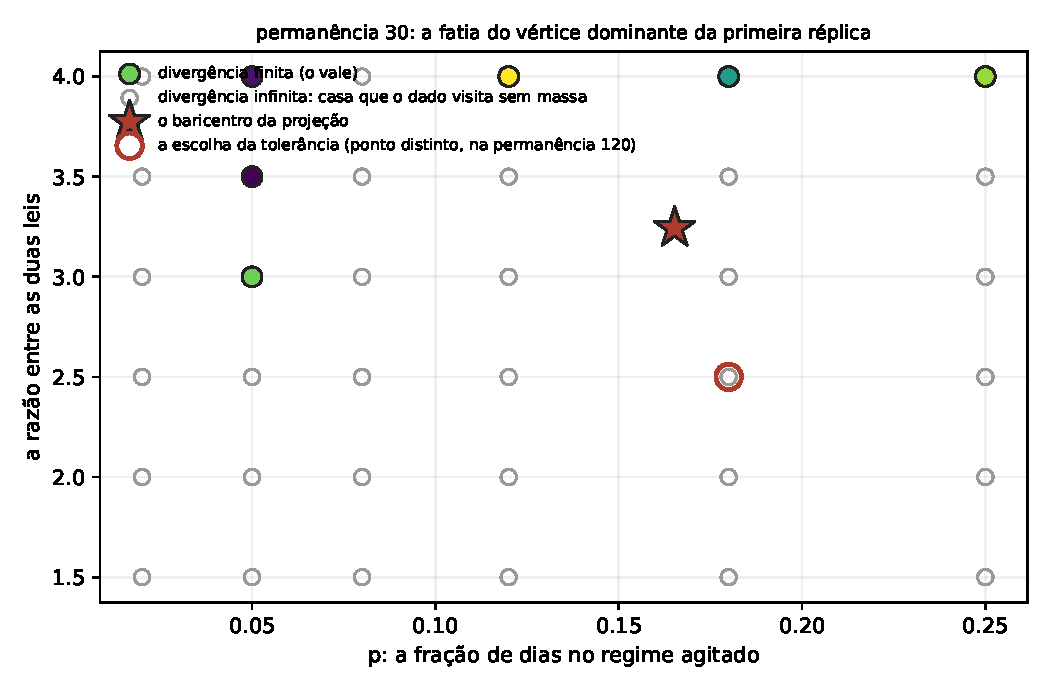
\includegraphics[width=\linewidth]{figuras/E47_projecao_1.pdf}
  \caption{O vale da divergência no plano da permanência, com a escolha da geometria (a estrela,
    com o peso do membro dominante) e a escolha da tolerância (os círculos abertos). Os dois
    critérios respondem a perguntas diferentes, e o desenho mostra que respondem com pontos
    diferentes.}
  \label{fig:projecao}
\end{figure}

\begin{figure}[htbp]
  \centering
  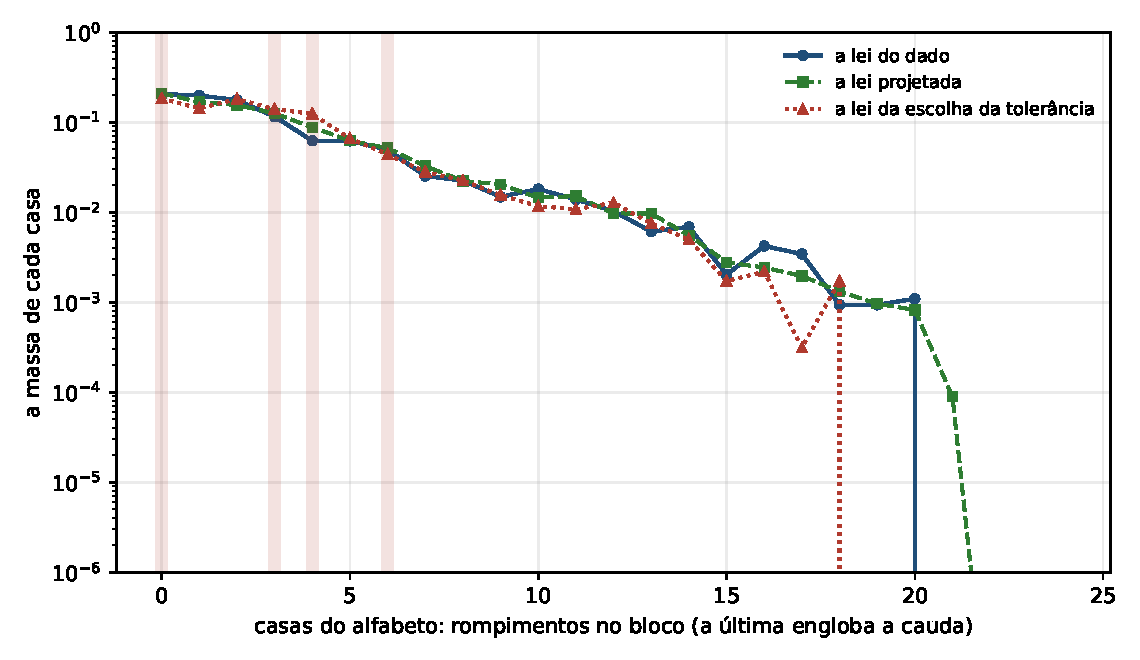
\includegraphics[width=\linewidth]{figuras/E47_projecao_2.pdf}
  \caption{As três leis sobre o alfabeto das contagens: o dado, a projeção e a escolha da
    tolerância. A escala é logarítmica porque a massa cai por décadas.}
  \label{fig:leis}
\end{figure}

O que fica desta seção não é que a geometria esteja certa e a tolerância errada. As duas
respondem a perguntas diferentes: a tolerância responde \emph{quais explicações as quatro
estatísticas admitem}, e a geometria responde \emph{qual lei desta família está mais perto da lei
que o dado mostrou} --- e é essa a pergunta que não tem alternativa canônica nenhuma. Nenhuma das
duas refuta: refutação é do dado, e as duas trabalham dentro da família que sobrou.

\section{O que fica}

Fica a \textbf{geometria}: uma família de explicações, um punhado de estatísticas, e o conjunto
dos membros que sobrevivem a todas. A taxa deixa uma região grande; o agrupamento dos dias ruins
corta essa mesma família a zero; a persistência a traz de volta, e as quatro estatísticas juntas
deixam duas explicações. Nenhuma delas é o ponto que uma medição sozinha promete.

E fica a disciplina que o capítulo repete de propósito: dizer "o modelo explica os dados" sem
dizer se o conjunto que sobra é uma região ou o vazio é uma frase sem conteúdo. Uma região
declarada é resultado; um vazio declarado é refutação; o resto é retórica\cite{ioannidis2005most}.

O fracasso seguinte não está na conta, está no material. Encolher a região com mais estatísticas
tem limite, porque as quatro que usei são todas do mesmo pedaço de passado, do mesmo mercado. E as
duas explicações que sobreviveram têm um buraco embaixo, maior que a região: ambas recebem a cauda
pronta --- cada uma arruma os dias ruins à sua maneira, e nenhuma diz por que eles são grandes. Antes
de acumular mundos novos, o material tem de ser interrogado: de onde vem a cauda que as duas usam
sem explicar? É essa a pergunta seguinte --- e a dos mundos novos espera por ela.
